% failuredetection.tex
\documentclass[dareport.tex]{subfiles}
\begin{document}
% Content here
\section{Failure Detection}

Initially, simple heartbeat is implemented in Strike Server. Each server will try to establish a short TCP connection to all peer severs for every T seconds. Each server maintains a data structure of hashmap to store error factor for all known servers. For example, if \verb|server 1| fails to establish connection with \verb|server 2|, \verb|server 1| will modify its local hashmap to increase the error factor of \verb|server 2| by 1. When the error factor of a particular server reaches F, that server is considered as crashed. (Parameter T and F can be set in configuration file) A server detecting any failed server will broadcast a message to all other servers to inform them deleting the failed server. This can be a problem in a partially connected network, a detected "fail server" will be remove from server list from all other servers since no consensus on deleting failure server is met. The consensus improvements will be discussed in consensus session.

Failure detection using simple heartbeat may works fine in a group of a few servers, however it is not effective when servers scale to a large number. For $N$ servers, there will be $O(N^{2})$ TCP connections among the servers for every heartbeat interval. This will lead to message explosion, which is described in "Failure Detectors for Large-Scale Distributed Systems". A good failure detector in large scale distributed system must prevent flooding or overloading the network with failure detection related messages whereas the current heartbeat failure detector does not.
To address this problem, we used gossip-type protocol to implement distributed algorithms in the chat system. In paper "Failure Detectors for Large-Scale Distributed Systems", it introduces a basic gossiping protocol, we used that as a baseline of implementing gossip algorithm on the chat system. Firstly, each server will run a failure detection module when it is started. We used Quartz Job Scheduling to run this module as a job since Strike is developed in Java. Each server maintains a hashmap data structure to store heartbeat counts for all known servers. i.e. \verb|{"sever1":0, "server2":2, "server3":1, "server4":2}|. In the paper, it 

\begin{figure}[h]
\label{fig:Gossip Module}
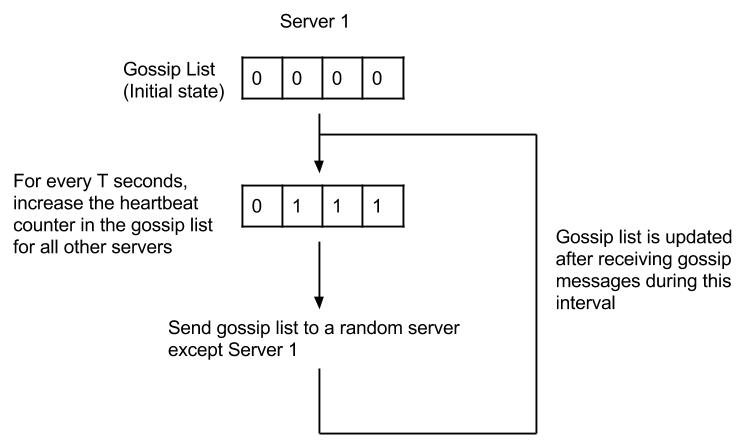
\includegraphics[scale=0.6]{gossip_send.jpg}
\caption{Gossip Module}
\centering
\end{figure}



\end{document}